% !TeX spellcheck = it_IT
\newpage
\section{Energia in un sistema ICT}
Prendiamo come riferimento il modello \textbf{olistico} di \emph{Drouant et al} proposto nel 2014.
\subsection{Energia}
L'energia si compone di:
\begin{equation}
	E = E_i + E_u + Ef
\end{equation}
dove:
\begin{itemize}
	\item \textbf{$E_i$} (iniziale) rappresenta l'energia necessaria per la \emph{progettazione} ($E_p$), \emph{produzione} ($E_m$) e \emph{trasporto al venditore} ($E_{ti}$)
	\item \textbf{$E_u$} (utilizzo) rappresenta l'energia necessaria per l'\emph{uso} e la \emph{gestione}
	\item \textbf{$E_f$} (finale) rappresenta l'energia necessaria al \emph{trasporto al centro di smaltimento} ($E_{tf}$) e il \emph{riciclo} ($E_r$)
\end{itemize}
Ottenendo quindi:
\begin{equation}
	E = (E_p + E_m + E_{ti}) + \int_{t=0}^{t=\text{fine vita}}P_u(t)dt + (E_{tf} + E_r)
\end{equation}
In particolare, l'integrale rappresenta la somma di quanto consuma in ogni istante di vita in un prodotto:
\begin{equation}
	\tilde{PUE} \cdot \int_{t=0}^{t=1_{year}} P_u(t)dt \simeq \tilde{PUE} \cdot \sum_{i \in S} \epsilon_i h_i
\end{equation}
ovvero il \emph{PUE} moltiplicato per la sommatoria della \textbf{potenza media oraria} moltiplicato per le \textbf{ore} di funzionamento annue di ogni elemento dell'insieme dei componenti hardware del sistema ($S$).\\

\subsection{Carbonio}
Per quanto riguarda invece l'emissione di $CO_2$ equivalente, la formula prevede, con terminologia analoga:
\begin{equation}
	C = C_i + C_u + C_f = (\frac{\alpha_p}{\tau_p} \cdot E_p + \frac{\alpha_m}{\tau_m} \cdot E_m + \frac{\alpha_{ti}}{\tau_{ti}} \cdot E_{ti}) + \frac{\alpha_u}{\tau_u} \cdot \int_{t=0}^{t=\text{fine vita}}P_u(t)dt + (\frac{\alpha_{tf}}{\tau_{tf}} \cdot E_{tf} + \frac{\alpha_r}{\tau_r} \cdot E_r)
\end{equation}
dove $\alpha_j$ rappresenta l'\textbf{intensità} di carbonio per la fase $j$, misurata in $\frac{g CO_2-eq}{KWh}$ mentre $\tau_j$ rappresenta l'\textbf{efficienza} dell'infrastruttura elettrica (e.g. in Europa $0.95$). Possiamo anche qui trasformare la formula come segue:
\begin{equation}
	C = C_i  + C_u + C_f = \sum_{S \in \{i,u,f\}} \frac{\alpha_S}{\tau_S} \cdot E_s = \frac{\alpha_i}{\tau_i} \cdot E_i + \frac{\alpha_u}{\tau_u} \cdot E_u + \frac{\alpha_f}{\tau_f} \cdot E_f
\end{equation}

\subsection{Componenti}
Il nostro sistema $S$ si compone di due parti:
\begin{equation}
	S = S_r \cup  \tilde{S_r}
\end{equation}
ovvero componenti \textbf{riusabili} e non. Di quelli non riusabili, una percentuale $p_i \in [0,1]$  rappresenta la parte \textbf{riciclabile}.

\subsection{Caso di studio}
Prendiamo come caso di studio una rete LAN che si connette ad un datacentre privato. Si vuole verificare quale delle tre architetture sotto fornisce:
\begin{itemize}
	\item \textbf{Riciclabilità} sopra al $70\%$
	\item \textbf{Emissioni} sono i $700 Kg$ lungo l'intero ciclo di vita
	\item \textbf{Performance}, ovvero probabilità di fallimento oraria, inferiore a $10^{-6}$
\end{itemize}
\begin{center}
	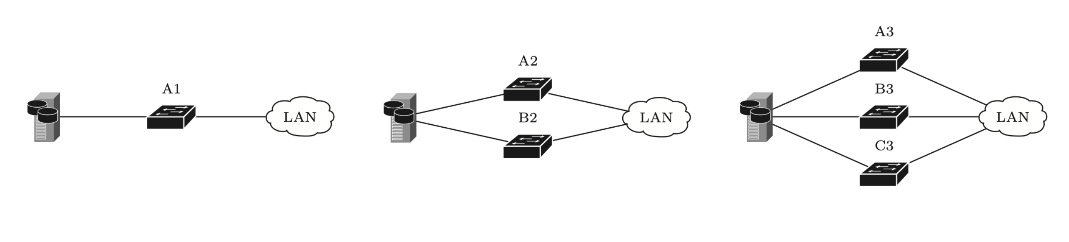
\includegraphics[scale=0.4]{study_case_model.png}
\end{center}
I dati del caso sono i seguenti:
\begin{itemize}
	\item Indici di \textbf{riciclabilità} $p_i$:
	\begin{itemize}
		\item \emph{Switch}: $0.7$
		\item \emph{Cavo}: $0.9$
	\end{itemize}
	dove durante il ciclo di vita un cavo e uno switch verranno sostituiti e alla fine i cavi saranno riusati e gli switch dismessi.
	\item \textbf{Potenza} assorbita da uno switch in un ciclo di vita di $3$ anni (con $\alpha = 0.389  \frac{kg CO_2-eq}{kWh}$):
	\begin{itemize}
		\item \emph{Costruzione} di uno switch $750kWh$ mentre di un cavo $1kWh$
		\item \emph{Smaltimento} di uno switch $400kWh$ mentre di un cavo $1kWh$
		\item \emph{Utilizzo} di uno switch $0.05kW$ da sommare a:
		\begin{itemize}
			\item $0.015kW$ per ogni porta usata al $100\%$ (porte 100 BaseT con uso medio di 10Mbps)
			\item $0.006kW$ per ogni porta idle 
		\end{itemize}
	\end{itemize}
	\item Probabilità di \textbf{fallimento} di uno switch o cavo ogni ora $10^{-5}$
	\item La \textbf{ridondanza} viene utilizzata solo quando necessario ed assumiamo quindi che sia sempre in idle
\end{itemize}
Di seguito lo svolgimento dei vari casi:
\begin{itemize}
	\item \textbf{Riciclabilità}
	\begin{equation*}
		\begin{split}
			& R_1 = \frac{0.7 + 0.7 +0.9}{3} = 0.767 = 76.7\%\\
			& R_2 = \frac{0.7+0.9 + 0.7 + 0.7}{4} = 0.75 = 75\% \\
			& R_3 = \frac{0.7 + 0.9 + 0.7 + 0.7 + 0.7}{5} = 0.74 = 74\%
		\end{split}
	\end{equation*}
	\newpage
	\item \textbf{Emissioni}
	\begin{itemize}
		\item Caso 1:
		\begin{equation*}
			\begin{split}
				& C_{switch_m} = 750kWh \cdot 2 \cdot \frac{0.389 \frac{kg CO_2-eq}{kWh}}{0.95} = 614.211 kg CO_w-eq\\
				& C_{switch_r} = 400 kWh \cdot 2 \cdot \frac{0.389 \frac{kg CO_2-eq}{kWh}}{0.95} = 327.579 kg CO_2-eq \\
				& C_{cavi_m} = 1kWh \cdot 3 \cdot \frac{0.389 \frac{kg CO_2-eq}{kWh}}{0.95}  = 1.228 kg CO_2-eq\\
				& C_{cavi_r} = 1kWh \cdot \frac{0.389 \frac{kg CO_2-eq}{kWh}}{0.95} = 0.409 kg CO_2-eq \\
				& C_{switch_u} = 0.015kW \cdot 2 \cdot \frac{0.389 \frac{kg CO_2-eq}{kWh}}{0.95} \cdot 8760\frac{h}{y} \cdot3y +\\
				 & + 0.05kW \cdot \frac{0.389 \frac{kg CO_2-eq}{kWh}}{0.95} \cdot 8760\frac{h}{y} \cdot 3 y= 860.877 kg CO_2-eq \\
				& C_{tot} = (614.211 + 327.579 + 1.228 + 0.409 + 860.877)kg CO_2-eq = \\
				& = 1804.304 kg CO_2-eq
			\end{split}
		\end{equation*}
		\item Caso 2:
		\begin{equation*}
			\begin{split}
				& C_{switch_m} = 750kWh \cdot 3 \cdot \frac{0.389 \frac{kg CO_2-eq}{kWh}}{0.95} = 921.316 kg CO_w-eq\\
				& C_{switch_r} = 400 kWh \cdot 3 \cdot \frac{0.389 \frac{kg CO_2-eq}{kWh}}{0.95} = 491.368 kg CO_2-eq \\
				& C_{cavi_m} = 1kWh \cdot 5 \cdot \frac{0.389 \frac{kg CO_2-eq}{kWh}}{0.95}  = 2.047 kg CO_2-eq\\
				& C_{cavi_r} = 1kWh \cdot \frac{0.389 \frac{kg CO_2-eq}{kWh}}{0.95} = 0.409 kg CO_2-eq \\
				& C_{switch_u} = 0.015kW \cdot 2 \cdot \frac{0.389 \frac{kg CO_2-eq}{kWh}}{0.95} \cdot 8760\frac{h}{y}\cdot 3y +\\
				& + 0.006kW \cdot 2 \cdot \frac{0.389 \frac{kg CO_2-eq}{kWh}}{0.95} \cdot 8760\frac{h}{y} \cdot 3y+ \\
				& + 0.05kW \cdot 2 \cdot \frac{0.389 \frac{kg CO_2-eq}{kWh}}{0.95} \cdot 8760\frac{h}{y} \cdot 3y= 1528.058 kg CO_2-eq \\
				& C_{tot} = (921.316 + 491.368 + 2.047 + 0.409 + 1528.058)kg CO_2-eq = \\
				& = 2943.198 kg CO_2-eq
			\end{split}
		\end{equation*}
		\item Caso 3:
		\begin{equation*}
			\begin{split}
				& C_{switch_m} = 750kWh \cdot 4 \cdot \frac{0.389 \frac{kg CO_2-eq}{kWh}}{0.95} = 1228.421 kg CO_w-eq\\
				& C_{switch_r} = 400 kWh \cdot 4 \cdot \frac{0.389 \frac{kg CO_2-eq}{kWh}}{0.95} = 655.158 kg CO_2-eq \\
				& C_{cavi_m} = 1kWh \cdot 7 \cdot \frac{0.389 \frac{kg CO_2-eq}{kWh}}{0.95}  = 2.866 kg CO_2-eq\\
				& C_{cavi_r} = 1kWh \cdot \frac{0.389 \frac{kg CO_2-eq}{kWh}}{0.95} = 0.409 kg CO_2-eq \\
				& C_{switch_u} = 0.015kW \cdot 2 \cdot \frac{0.389 \frac{kg CO_2-eq}{kWh}}{0.95} \cdot 8760\frac{h}{y} \cdot 3y+\\
				&+ 0.006kW \cdot 4 \cdot \frac{0.389 \frac{kg CO_2-eq}{kWh}}{0.95} \cdot 8760\frac{h}{y} \cdot 3y+ \\
				& + 0.05kW \cdot 3 \cdot \frac{0.389 \frac{kg CO_2-eq}{kWh}}{0.95} \cdot 8760\frac{h}{y} \cdot 3y= 2195.238 kg CO_2-eq \\
				& C_{tot} = (1228.421 + 655.158 + 2.866 + 0.409 + 2195.238)kg CO_2-eq =\\
				& = 4082.092 kg CO_2-eq
			\end{split}
		\end{equation*}
	\end{itemize}
	\item \textbf{Performance}: la probabilità che il sistema funzioni è
	\begin{equation*}
		(1-10^{-5})^3 = 0.99997
	\end{equation*}
	e quindi:
	\begin{equation*}
		\begin{split}
			& P_1 = (1-0.99997)^1 = 3 \cdot 10^{-5}\\
			& P_2 = (1-0.99997)^2 = 9 \cdot 10^{-10} \\
			& P_3 =(1-0.99997)^3 = 2.7 \cdot 10^{-14}
		\end{split}
	\end{equation*}
\end{itemize}
Concludendo, tutte le configurazioni rispettano il punto sulla \emph{riciclabilità}, nessuna quello sulle \emph{emissioni} e solo le ultime due quello sull'\emph{affidabilità}.